Afin d'accomplir ce projet avec succès, nous avons opté pour une approche intégrant des
\textbf{analyses théoriques}, la \textbf{mise en oeuvre d'algorithmes} et des \textbf{évaluations
empiriques}\footnote{L'évaluation empirique désigne le processus consistant à utiliser des 
expériences, des mesures et des observations pour évaluer la performance ou l'efficacité 
d'un système ou d'une approche particulière}. Pour ce faire, nous devrions dans un premier temps
fixer des objectifs clairs et définir les différentes étapes de notre travail. Ensuite, nous devrions
nous pencher sur la relation de ces derniers en s'organisant et en planifiant notre travail.

\subsection{Etapes du projet}
Notre travail est divisé en trois grandes étapes principales :
\begin{itemize}
	\item \textbf{Planification} :  Définition des questions de recherche, formulation des hypothèses, Recherche bibliographique, choix de l'approche méthodologique et modèlisation du jeu.
	\item \textbf{Implémentation et Développement}: Développement du jeu, implémentation des algorithmes de recherche adversarial et des heuristiques, préparation des données et des expériences.
	\item \textbf{Evaluation et Analyse}: Analyse des résultats, interprétation des résultats et discussion des résultats.
\end{itemize}
Chacune des étapes comporte des objectifs et tâches spécifiques dont leur accomplissement est 
nécessaire pour le succès du projet.

\subsection{Gestion du projet}

Pour le bon déroulement du projet, nous avons décidé d'organiser globalement divers parties implémenter par chaque membre du groupe. 
Ainsi, nous avons décidé de nous répartir les tâches suivantes:
\begin{itemize}
	\item \textbf{Manne}: Implémentation du modèle de jeu et des heuristiques
	\item \textbf{Amirath}: Implémentation des algorithmes de recherche adversarial ($Max^n$ et $Paranoid$)
	\item \textbf{Catherine}: Implémentation des algorithmes de recherche adversarial et mise en place de la plateforme de test
	\item \textbf{Sekou} : Réalisation de l'interface graphique
\end{itemize}
En outre, nous avons décidé que chacun des membres du groupe devrait participer à l'analyse des résultats.
\subsection{Planification du travail}
Le diagramme de Gantt\footnote{Diagramme de Gantt est un diagramme de type barre qui permet de représenter graphiquement l'avancement d'un projet.} ci-dessous représente la planification du travail.
\begin{figure}[!ht]
	\centering
	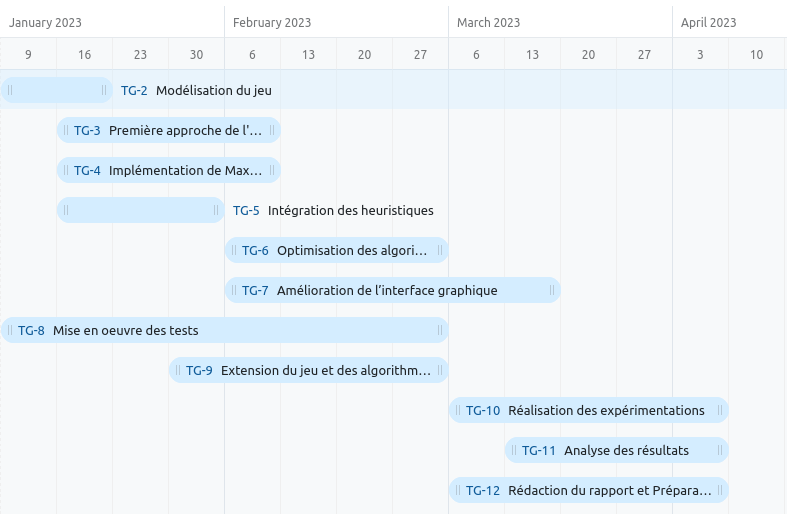
\includegraphics[scale=0.5]{Images/gant.png}
	\caption{Diagramme de Gantt}
	\label{fig:gantt}
\end{figure}
Nous avons décidé de travailler sur le projet en trois phases, à savoir:
\begin{itemize}
	\item \textbf{Phase 1}: Développement de l'environnement de jeu, implémentation des heuristiques, des algorithmes de recherche adversarial et mise en place de la plateforme de test
	\item \textbf{Phase 2}: Amélioration de l'environnement de jeu, algorithmes et extensions des algorithmes à la version multi-joueurs
	\item \textbf{Phase 3}: Réalisation des expériences et analyse des résultats
\end{itemize}
